\documentclass[1p]{elsarticle_modified}
%\bibliographystyle{elsarticle-num}

%\usepackage[colorlinks]{hyperref}
%\usepackage{abbrmath_seonhwa} %\Abb, \Ascr, \Acal ,\Abf, \Afrak
\usepackage{amsfonts}
\usepackage{amssymb}
\usepackage{amsmath}
\usepackage{amsthm}
\usepackage{scalefnt}
\usepackage{amsbsy}
\usepackage{kotex}
\usepackage{caption}
\usepackage{subfig}
\usepackage{color}
\usepackage{graphicx}
\usepackage{xcolor} %% white, black, red, green, blue, cyan, magenta, yellow
\usepackage{float}
\usepackage{setspace}
\usepackage{hyperref}

\usepackage{tikz}
\usetikzlibrary{arrows}

\usepackage{multirow}
\usepackage{array} % fixed length table
\usepackage{hhline}

%%%%%%%%%%%%%%%%%%%%%
\makeatletter
\renewcommand*\env@matrix[1][\arraystretch]{%
	\edef\arraystretch{#1}%
	\hskip -\arraycolsep
	\let\@ifnextchar\new@ifnextchar
	\array{*\c@MaxMatrixCols c}}
\makeatother %https://tex.stackexchange.com/questions/14071/how-can-i-increase-the-line-spacing-in-a-matrix
%%%%%%%%%%%%%%%

\usepackage[normalem]{ulem}

\newcommand{\msout}[1]{\ifmmode\text{\sout{\ensuremath{#1}}}\else\sout{#1}\fi}
%SOURCE: \msout is \stkout macro in https://tex.stackexchange.com/questions/20609/strikeout-in-math-mode

\newcommand{\cancel}[1]{
	\ifmmode
	{\color{red}\msout{#1}}
	\else
	{\color{red}\sout{#1}}
	\fi
}

\newcommand{\add}[1]{
	{\color{blue}\uwave{#1}}
}

\newcommand{\replace}[2]{
	\ifmmode
	{\color{red}\msout{#1}}{\color{blue}\uwave{#2}}
	\else
	{\color{red}\sout{#1}}{\color{blue}\uwave{#2}}
	\fi
}

\newcommand{\Sol}{\mathcal{S}} %segment
\newcommand{\D}{D} %diagram
\newcommand{\A}{\mathcal{A}} %arc


%%%%%%%%%%%%%%%%%%%%%%%%%%%%%5 test

\def\sl{\operatorname{\textup{SL}}(2,\Cbb)}
\def\psl{\operatorname{\textup{PSL}}(2,\Cbb)}
\def\quan{\mkern 1mu \triangleright \mkern 1mu}

\theoremstyle{definition}
\newtheorem{thm}{Theorem}[section]
\newtheorem{prop}[thm]{Proposition}
\newtheorem{lem}[thm]{Lemma}
\newtheorem{ques}[thm]{Question}
\newtheorem{cor}[thm]{Corollary}
\newtheorem{defn}[thm]{Definition}
\newtheorem{exam}[thm]{Example}
\newtheorem{rmk}[thm]{Remark}
\newtheorem{alg}[thm]{Algorithm}

\newcommand{\I}{\sqrt{-1}}
\begin{document}

%\begin{frontmatter}
%
%\title{Boundary parabolic representations of knots up to 8 crossings}
%
%%% Group authors per affiliation:
%\author{Yunhi Cho} 
%\address{Department of Mathematics, University of Seoul, Seoul, Korea}
%\ead{yhcho@uos.ac.kr}
%
%
%\author{Seonhwa Kim} %\fnref{s_kim}}
%\address{Center for Geometry and Physics, Institute for Basic Science, Pohang, 37673, Korea}
%\ead{ryeona17@ibs.re.kr}
%
%\author{Hyuk Kim}
%\address{Department of Mathematical Sciences, Seoul National University, Seoul 08826, Korea}
%\ead{hyukkim@snu.ac.kr}
%
%\author{Seokbeom Yoon}
%\address{Department of Mathematical Sciences, Seoul National University, Seoul, 08826,  Korea}
%\ead{sbyoon15@snu.ac.kr}
%
%\begin{abstract}
%We find all boundary parabolic representation of knots up to 8 crossings.
%
%\end{abstract}
%\begin{keyword}
%    \MSC[2010] 57M25 
%\end{keyword}
%
%\end{frontmatter}

%\linenumbers
%\tableofcontents
%
\newcommand\colored[1]{\textcolor{white}{\rule[-0.35ex]{0.8em}{1.4ex}}\kern-0.8em\color{red} #1}%
%\newcommand\colored[1]{\textcolor{white}{ #1}\kern-2.17ex	\textcolor{white}{ #1}\kern-1.81ex	\textcolor{white}{ #1}\kern-2.15ex\color{red}#1	}

{\Large $\underline{12a_{0081}~(K12a_{0081})}$}

\setlength{\tabcolsep}{10pt}
\renewcommand{\arraystretch}{1.6}
\vspace{1cm}\begin{tabular}{m{100pt}>{\centering\arraybackslash}m{274pt}}
\multirow{5}{120pt}{
	\centering
	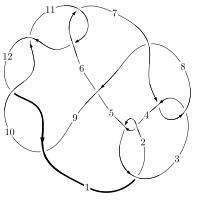
\includegraphics[width=112pt]{../../../GIT/diagram.site/Diagrams/png/882_12a_0081.png}\\
\ \ \ A knot diagram\footnotemark}&
\allowdisplaybreaks
\textbf{Linearized knot diagam} \\
\cline{2-2}
 &
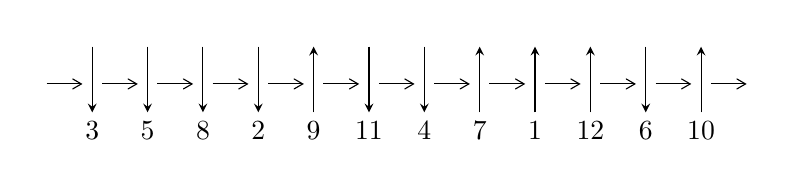
\begin{tikzpicture}[x=20pt, y=17pt]
	% nodes
	\node (C0) at (0, 0) {};
	\node (C1) at (1, 0) {};
	\node (C1U) at (1, +1) {};
	\node (C1D) at (1, -1) {3};

	\node (C2) at (2, 0) {};
	\node (C2U) at (2, +1) {};
	\node (C2D) at (2, -1) {5};

	\node (C3) at (3, 0) {};
	\node (C3U) at (3, +1) {};
	\node (C3D) at (3, -1) {8};

	\node (C4) at (4, 0) {};
	\node (C4U) at (4, +1) {};
	\node (C4D) at (4, -1) {2};

	\node (C5) at (5, 0) {};
	\node (C5U) at (5, +1) {};
	\node (C5D) at (5, -1) {9};

	\node (C6) at (6, 0) {};
	\node (C6U) at (6, +1) {};
	\node (C6D) at (6, -1) {11};

	\node (C7) at (7, 0) {};
	\node (C7U) at (7, +1) {};
	\node (C7D) at (7, -1) {4};

	\node (C8) at (8, 0) {};
	\node (C8U) at (8, +1) {};
	\node (C8D) at (8, -1) {7};

	\node (C9) at (9, 0) {};
	\node (C9U) at (9, +1) {};
	\node (C9D) at (9, -1) {1};

	\node (C10) at (10, 0) {};
	\node (C10U) at (10, +1) {};
	\node (C10D) at (10, -1) {12};

	\node (C11) at (11, 0) {};
	\node (C11U) at (11, +1) {};
	\node (C11D) at (11, -1) {6};

	\node (C12) at (12, 0) {};
	\node (C12U) at (12, +1) {};
	\node (C12D) at (12, -1) {10};
	\node (C13) at (13, 0) {};

	% arrows
	\draw[->,>={angle 60}]
	(C0) edge (C1) (C1) edge (C2) (C2) edge (C3) (C3) edge (C4) (C4) edge (C5) (C5) edge (C6) (C6) edge (C7) (C7) edge (C8) (C8) edge (C9) (C9) edge (C10) (C10) edge (C11) (C11) edge (C12) (C12) edge (C13) ;	\draw[->,>=stealth]
	(C1U) edge (C1D) (C2U) edge (C2D) (C3U) edge (C3D) (C4U) edge (C4D) (C5D) edge (C5U) (C6U) edge (C6D) (C7U) edge (C7D) (C8D) edge (C8U) (C9D) edge (C9U) (C10D) edge (C10U) (C11U) edge (C11D) (C12D) edge (C12U) ;
	\end{tikzpicture} \\
\hhline{~~} \\& 
\textbf{Solving Sequence} \\ \cline{2-2} 
 &
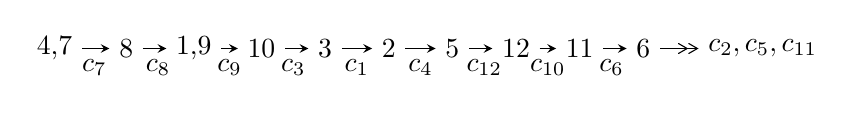
\begin{tikzpicture}[x=23pt, y=7pt]
	% node
	\node (A0) at (-1/8, 0) {4,7};
	\node (A1) at (1, 0) {8};
	\node (A2) at (33/16, 0) {1,9};
	\node (A3) at (25/8, 0) {10};
	\node (A4) at (33/8, 0) {3};
	\node (A5) at (41/8, 0) {2};
	\node (A6) at (49/8, 0) {5};
	\node (A7) at (57/8, 0) {12};
	\node (A8) at (65/8, 0) {11};
	\node (A9) at (73/8, 0) {6};
	\node (C1) at (1/2, -1) {$c_{7}$};
	\node (C2) at (3/2, -1) {$c_{8}$};
	\node (C3) at (21/8, -1) {$c_{9}$};
	\node (C4) at (29/8, -1) {$c_{3}$};
	\node (C5) at (37/8, -1) {$c_{1}$};
	\node (C6) at (45/8, -1) {$c_{4}$};
	\node (C7) at (53/8, -1) {$c_{12}$};
	\node (C8) at (61/8, -1) {$c_{10}$};
	\node (C9) at (69/8, -1) {$c_{6}$};
	\node (A10) at (11, 0) {$c_{2},c_{5},c_{11}$};

	% edge
	\draw[->,>=stealth]	
	(A0) edge (A1) (A1) edge (A2) (A2) edge (A3) (A3) edge (A4) (A4) edge (A5) (A5) edge (A6) (A6) edge (A7) (A7) edge (A8) (A8) edge (A9) ;
	\draw[->>,>={angle 60}]	
	(A9) edge (A10);
\end{tikzpicture} \\ 

\end{tabular} \\

\footnotetext{
The image of knot diagram is generated by the software ``\textbf{Draw programme}" developed by Andrew Bartholomew(\url{http://www.layer8.co.uk/maths/draw/index.htm\#Running-draw}), where we modified some parts for our purpose(\url{https://github.com/CATsTAILs/LinksPainter}).
}\phantom \\ \newline 
\centering \textbf{Ideals for irreducible components\footnotemark of $X_{\text{par}}$} 
 
\begin{align*}
I^u_{1}&=\langle 
-4.57817\times10^{68} u^{82}-4.41680\times10^{68} u^{81}+\cdots+1.40607\times10^{69} b-1.45069\times10^{70},\\
\phantom{I^u_{1}}&\phantom{= \langle  }-8.02816\times10^{70} u^{82}-7.69195\times10^{70} u^{81}+\cdots+1.71541\times10^{71} a-8.36164\times10^{71},\\
\phantom{I^u_{1}}&\phantom{= \langle  }u^{83}+u^{82}+\cdots+24 u+16\rangle \\
\\
I^v_{1}&=\langle 
a,\;- v^3+2 v^2+b-3 v+1,\;v^4-2 v^3+3 v^2- v+1\rangle \\
\end{align*}
\raggedright * 2 irreducible components of $\dim_{\mathbb{C}}=0$, with total 87 representations.\\
\footnotetext{All coefficients of polynomials are rational numbers. But the coefficients are sometimes approximated in decimal forms when there is not enough margin.}
\newpage
\renewcommand{\arraystretch}{1}
\centering \section*{I. $I^u_{1}= \langle -4.58\times10^{68} u^{82}-4.42\times10^{68} u^{81}+\cdots+1.41\times10^{69} b-1.45\times10^{70},\;-8.03\times10^{70} u^{82}-7.69\times10^{70} u^{81}+\cdots+1.72\times10^{71} a-8.36\times10^{71},\;u^{83}+u^{82}+\cdots+24 u+16 \rangle$}
\flushleft \textbf{(i) Arc colorings}\\
\begin{tabular}{m{7pt} m{180pt} m{7pt} m{180pt} }
\flushright $a_{4}=$&$\begin{pmatrix}0\\u\end{pmatrix}$ \\
\flushright $a_{7}=$&$\begin{pmatrix}1\\0\end{pmatrix}$ \\
\flushright $a_{8}=$&$\begin{pmatrix}1\\u^2\end{pmatrix}$ \\
\flushright $a_{1}=$&$\begin{pmatrix}0.468003 u^{82}+0.448403 u^{81}+\cdots+25.8370 u+4.87443\\0.325600 u^{82}+0.314123 u^{81}+\cdots+27.3694 u+10.3173\end{pmatrix}$ \\
\flushright $a_{9}=$&$\begin{pmatrix}u^2+1\\u^2\end{pmatrix}$ \\
\flushright $a_{10}=$&$\begin{pmatrix}-0.300402 u^{82}-0.851248 u^{81}+\cdots-25.8721 u-4.83081\\-0.617837 u^{82}-0.388150 u^{81}+\cdots-21.4249 u+11.7726\end{pmatrix}$ \\
\flushright $a_{3}=$&$\begin{pmatrix}u\\u^3+u\end{pmatrix}$ \\
\flushright $a_{2}=$&$\begin{pmatrix}0.518352 u^{82}+0.412444 u^{81}+\cdots+28.9820 u+7.48317\\0.507921 u^{82}+0.442205 u^{81}+\cdots+31.7802 u+14.3070\end{pmatrix}$ \\
\flushright $a_{5}=$&$\begin{pmatrix}-0.0480076 u^{82}+0.115039 u^{81}+\cdots+8.55001 u+5.12927\\0.419995 u^{82}+0.563442 u^{81}+\cdots+34.3871 u+10.0037\end{pmatrix}$ \\
\flushright $a_{12}=$&$\begin{pmatrix}-0.535339 u^{82}-0.604770 u^{81}+\cdots-41.7844 u-16.0490\\0.173440 u^{82}-0.441183 u^{81}+\cdots-33.7669 u-28.0780\end{pmatrix}$ \\
\flushright $a_{11}=$&$\begin{pmatrix}1.16268 u^{82}+0.674679 u^{81}+\cdots+49.5790 u-5.78307\\0.545400 u^{82}+0.632005 u^{81}+\cdots+36.8130 u+12.6970\end{pmatrix}$ \\
\flushright $a_{6}=$&$\begin{pmatrix}0.340652 u^{82}+0.495917 u^{81}+\cdots+30.9853 u+15.6302\\0.483055 u^{82}+0.630197 u^{81}+\cdots+29.4529 u+10.1873\end{pmatrix}$\\&\end{tabular}
\flushleft \textbf{(ii) Obstruction class $= -1$}\\~\\
\flushleft \textbf{(iii) Cusp Shapes $= -1.97759 u^{82}-1.33141 u^{81}+\cdots-38.4761 u+8.31564$}\\~\\
\newpage\renewcommand{\arraystretch}{1}
\flushleft \textbf{(iv) u-Polynomials at the component}\newline \\
\begin{tabular}{m{50pt}|m{274pt}}
Crossings & \hspace{64pt}u-Polynomials at each crossing \\
\hline $$\begin{aligned}c_{1}\end{aligned}$$&$\begin{aligned}
&u^{83}+45 u^{82}+\cdots+4 u+1
\end{aligned}$\\
\hline $$\begin{aligned}c_{2},c_{4}\end{aligned}$$&$\begin{aligned}
&u^{83}-5 u^{82}+\cdots-6 u+1
\end{aligned}$\\
\hline $$\begin{aligned}c_{3},c_{7}\end{aligned}$$&$\begin{aligned}
&u^{83}+u^{82}+\cdots+24 u+16
\end{aligned}$\\
\hline $$\begin{aligned}c_{5}\end{aligned}$$&$\begin{aligned}
&u^{83}+2 u^{82}+\cdots+15190 u+7769
\end{aligned}$\\
\hline $$\begin{aligned}c_{6},c_{11}\end{aligned}$$&$\begin{aligned}
&u^{83}+2 u^{82}+\cdots+2 u+1
\end{aligned}$\\
\hline $$\begin{aligned}c_{8}\end{aligned}$$&$\begin{aligned}
&u^{83}-27 u^{82}+\cdots-5056 u+256
\end{aligned}$\\
\hline $$\begin{aligned}c_{9},c_{10},c_{12}\end{aligned}$$&$\begin{aligned}
&u^{83}-20 u^{82}+\cdots+6 u+1
\end{aligned}$\\
\hline
\end{tabular}\\~\\
\newpage\renewcommand{\arraystretch}{1}
\flushleft \textbf{(v) Riley Polynomials at the component}\newline \\
\begin{tabular}{m{50pt}|m{274pt}}
Crossings & \hspace{64pt}Riley Polynomials at each crossing \\
\hline $$\begin{aligned}c_{1}\end{aligned}$$&$\begin{aligned}
&y^{83}-9 y^{82}+\cdots+44 y-1
\end{aligned}$\\
\hline $$\begin{aligned}c_{2},c_{4}\end{aligned}$$&$\begin{aligned}
&y^{83}-45 y^{82}+\cdots+4 y-1
\end{aligned}$\\
\hline $$\begin{aligned}c_{3},c_{7}\end{aligned}$$&$\begin{aligned}
&y^{83}+27 y^{82}+\cdots-5056 y-256
\end{aligned}$\\
\hline $$\begin{aligned}c_{5}\end{aligned}$$&$\begin{aligned}
&y^{83}+28 y^{82}+\cdots+953082182 y-60357361
\end{aligned}$\\
\hline $$\begin{aligned}c_{6},c_{11}\end{aligned}$$&$\begin{aligned}
&y^{83}+20 y^{82}+\cdots+6 y-1
\end{aligned}$\\
\hline $$\begin{aligned}c_{8}\end{aligned}$$&$\begin{aligned}
&y^{83}+51 y^{82}+\cdots+1724416 y-65536
\end{aligned}$\\
\hline $$\begin{aligned}c_{9},c_{10},c_{12}\end{aligned}$$&$\begin{aligned}
&y^{83}+88 y^{82}+\cdots+190 y-1
\end{aligned}$\\
\hline
\end{tabular}\\~\\
\newpage\flushleft \textbf{(vi) Complex Volumes and Cusp Shapes}
$$\begin{array}{c|c|c}  
\text{Solutions to }I^u_{1}& \I (\text{vol} + \sqrt{-1}CS) & \text{Cusp shape}\\
 \hline 
\begin{aligned}
u &= -0.625725 + 0.803794 I \\
a &= \phantom{-}0.95593 - 1.78325 I \\
b &= -0.809211 - 0.773750 I\end{aligned}
 & -2.81993 + 3.24237 I & \phantom{-0.000000 } 0 \\ \hline\begin{aligned}
u &= -0.625725 - 0.803794 I \\
a &= \phantom{-}0.95593 + 1.78325 I \\
b &= -0.809211 + 0.773750 I\end{aligned}
 & -2.81993 - 3.24237 I & \phantom{-0.000000 } 0 \\ \hline\begin{aligned}
u &= \phantom{-}0.823326 + 0.601133 I \\
a &= \phantom{-}0.994172 + 0.602548 I \\
b &= \phantom{-}0.97443 + 1.36618 I\end{aligned}
 & -7.35489 + 5.05736 I & \phantom{-0.000000 } 0 \\ \hline\begin{aligned}
u &= \phantom{-}0.823326 - 0.601133 I \\
a &= \phantom{-}0.994172 - 0.602548 I \\
b &= \phantom{-}0.97443 - 1.36618 I\end{aligned}
 & -7.35489 - 5.05736 I & \phantom{-0.000000 } 0 \\ \hline\begin{aligned}
u &= -0.811916 + 0.631020 I \\
a &= -0.985111 + 0.659411 I \\
b &= -0.84786 + 1.43938 I\end{aligned}
 & -7.63827 + 1.26608 I & \phantom{-0.000000 } 0 \\ \hline\begin{aligned}
u &= -0.811916 - 0.631020 I \\
a &= -0.985111 - 0.659411 I \\
b &= -0.84786 - 1.43938 I\end{aligned}
 & -7.63827 - 1.26608 I & \phantom{-0.000000 } 0 \\ \hline\begin{aligned}
u &= -0.133744 + 1.033610 I \\
a &= -0.235231 + 0.258306 I \\
b &= \phantom{-}0.952290 + 0.214525 I\end{aligned}
 & \phantom{-}2.24045 + 2.24996 I & \phantom{-0.000000 } 0 \\ \hline\begin{aligned}
u &= -0.133744 - 1.033610 I \\
a &= -0.235231 - 0.258306 I \\
b &= \phantom{-}0.952290 - 0.214525 I\end{aligned}
 & \phantom{-}2.24045 - 2.24996 I & \phantom{-0.000000 } 0 \\ \hline\begin{aligned}
u &= \phantom{-}0.718219 + 0.755764 I \\
a &= -1.01018 - 1.43608 I \\
b &= \phantom{-}0.328670 - 1.008960 I\end{aligned}
 & -4.52117 + 0.45961 I & \phantom{-0.000000 } 0 \\ \hline\begin{aligned}
u &= \phantom{-}0.718219 - 0.755764 I \\
a &= -1.01018 + 1.43608 I \\
b &= \phantom{-}0.328670 + 1.008960 I\end{aligned}
 & -4.52117 - 0.45961 I & \phantom{-0.000000 } 0\\
 \hline 
 \end{array}$$\newpage$$\begin{array}{c|c|c}  
\text{Solutions to }I^u_{1}& \I (\text{vol} + \sqrt{-1}CS) & \text{Cusp shape}\\
 \hline 
\begin{aligned}
u &= -0.583379 + 0.744333 I \\
a &= -0.599499 + 0.857080 I \\
b &= -0.084857 + 0.949548 I\end{aligned}
 & -1.06506 + 1.56831 I & -4.77521 - 3.38157 I \\ \hline\begin{aligned}
u &= -0.583379 - 0.744333 I \\
a &= -0.599499 - 0.857080 I \\
b &= -0.084857 - 0.949548 I\end{aligned}
 & -1.06506 - 1.56831 I & -4.77521 + 3.38157 I \\ \hline\begin{aligned}
u &= -0.699113 + 0.817903 I \\
a &= \phantom{-}1.03783 - 1.03599 I \\
b &= \phantom{-}1.03036 - 1.77245 I\end{aligned}
 & -10.88710 - 1.33695 I & \phantom{-0.000000 } 0 \\ \hline\begin{aligned}
u &= -0.699113 - 0.817903 I \\
a &= \phantom{-}1.03783 + 1.03599 I \\
b &= \phantom{-}1.03036 + 1.77245 I\end{aligned}
 & -10.88710 + 1.33695 I & \phantom{-0.000000 } 0 \\ \hline\begin{aligned}
u &= -0.761911 + 0.520219 I \\
a &= \phantom{-}0.419807 - 0.889805 I \\
b &= \phantom{-}0.245481 - 0.220375 I\end{aligned}
 & -0.709170 - 1.043470 I & \phantom{-0.000000 -}     -6
0. 10   + 0.525052 I \\ \hline\begin{aligned}
u &= -0.761911 - 0.520219 I \\
a &= \phantom{-}0.419807 + 0.889805 I \\
b &= \phantom{-}0.245481 + 0.220375 I\end{aligned}
 & -0.709170 + 1.043470 I & \phantom{-0.000000 }      -6
0. 10   - 0.525052 I \\ \hline\begin{aligned}
u &= \phantom{-}0.843982 + 0.682431 I \\
a &= -1.033390 - 0.928808 I \\
b &= -0.476474 - 1.005040 I\end{aligned}
 & -4.36263 + 2.17365 I & \phantom{-0.000000 } 0 \\ \hline\begin{aligned}
u &= \phantom{-}0.843982 - 0.682431 I \\
a &= -1.033390 + 0.928808 I \\
b &= -0.476474 + 1.005040 I\end{aligned}
 & -4.36263 - 2.17365 I & \phantom{-0.000000 } 0 \\ \hline\begin{aligned}
u &= -0.894299 + 0.161895 I \\
a &= -0.276725 - 0.077384 I \\
b &= -0.201389 + 0.785138 I\end{aligned}
 & -5.54438 + 1.11456 I & -5.40813 + 0.61307 I \\ \hline\begin{aligned}
u &= -0.894299 - 0.161895 I \\
a &= -0.276725 + 0.077384 I \\
b &= -0.201389 - 0.785138 I\end{aligned}
 & -5.54438 - 1.11456 I & -5.40813 - 0.61307 I\\
 \hline 
 \end{array}$$\newpage$$\begin{array}{c|c|c}  
\text{Solutions to }I^u_{1}& \I (\text{vol} + \sqrt{-1}CS) & \text{Cusp shape}\\
 \hline 
\begin{aligned}
u &= \phantom{-}0.899076 + 0.117669 I \\
a &= \phantom{-}0.356440 - 0.034756 I \\
b &= \phantom{-}0.361343 + 0.806350 I\end{aligned}
 & -5.43027 + 4.95461 I & -4.96710 - 6.01399 I \\ \hline\begin{aligned}
u &= \phantom{-}0.899076 - 0.117669 I \\
a &= \phantom{-}0.356440 + 0.034756 I \\
b &= \phantom{-}0.361343 - 0.806350 I\end{aligned}
 & -5.43027 - 4.95461 I & -4.96710 + 6.01399 I \\ \hline\begin{aligned}
u &= \phantom{-}0.482182 + 0.982828 I \\
a &= \phantom{-}0.288985 + 1.186530 I \\
b &= -0.515329 + 0.386646 I\end{aligned}
 & \phantom{-}3.22997 - 1.59915 I & \phantom{-0.000000 } 0 \\ \hline\begin{aligned}
u &= \phantom{-}0.482182 - 0.982828 I \\
a &= \phantom{-}0.288985 - 1.186530 I \\
b &= -0.515329 - 0.386646 I\end{aligned}
 & \phantom{-}3.22997 + 1.59915 I & \phantom{-0.000000 } 0 \\ \hline\begin{aligned}
u &= \phantom{-}0.711300 + 0.832616 I \\
a &= -1.01619 - 1.09996 I \\
b &= -0.88624 - 1.84707 I\end{aligned}
 & -11.15090 - 5.10243 I & \phantom{-0.000000 } 0 \\ \hline\begin{aligned}
u &= \phantom{-}0.711300 - 0.832616 I \\
a &= -1.01619 + 1.09996 I \\
b &= -0.88624 + 1.84707 I\end{aligned}
 & -11.15090 + 5.10243 I & \phantom{-0.000000 } 0 \\ \hline\begin{aligned}
u &= -0.615819 + 0.910490 I \\
a &= \phantom{-}0.610401 - 0.943583 I \\
b &= \phantom{-}0.554605 - 0.956704 I\end{aligned}
 & -2.48058 + 1.63613 I & \phantom{-0.000000 } 0 \\ \hline\begin{aligned}
u &= -0.615819 - 0.910490 I \\
a &= \phantom{-}0.610401 + 0.943583 I \\
b &= \phantom{-}0.554605 + 0.956704 I\end{aligned}
 & -2.48058 - 1.63613 I & \phantom{-0.000000 } 0 \\ \hline\begin{aligned}
u &= \phantom{-}0.177547 + 1.086860 I \\
a &= -0.252176 + 0.904141 I \\
b &= \phantom{-}0.383665 - 0.271787 I\end{aligned}
 & -1.02878 + 1.71356 I & \phantom{-0.000000 } 0 \\ \hline\begin{aligned}
u &= \phantom{-}0.177547 - 1.086860 I \\
a &= -0.252176 - 0.904141 I \\
b &= \phantom{-}0.383665 + 0.271787 I\end{aligned}
 & -1.02878 - 1.71356 I & \phantom{-0.000000 } 0\\
 \hline 
 \end{array}$$\newpage$$\begin{array}{c|c|c}  
\text{Solutions to }I^u_{1}& \I (\text{vol} + \sqrt{-1}CS) & \text{Cusp shape}\\
 \hline 
\begin{aligned}
u &= -0.907958 + 0.636974 I \\
a &= \phantom{-}1.005050 - 0.653160 I \\
b &= \phantom{-}0.911110 - 0.798415 I\end{aligned}
 & -2.46547 - 5.87569 I & \phantom{-0.000000 } 0 \\ \hline\begin{aligned}
u &= -0.907958 - 0.636974 I \\
a &= \phantom{-}1.005050 + 0.653160 I \\
b &= \phantom{-}0.911110 + 0.798415 I\end{aligned}
 & -2.46547 + 5.87569 I & \phantom{-0.000000 } 0 \\ \hline\begin{aligned}
u &= \phantom{-}0.042401 + 1.116900 I \\
a &= \phantom{-}0.433979 + 0.466369 I \\
b &= -0.986304 - 0.010974 I\end{aligned}
 & \phantom{-}5.17570 + 0.24359 I & \phantom{-0.000000 } 0 \\ \hline\begin{aligned}
u &= \phantom{-}0.042401 - 1.116900 I \\
a &= \phantom{-}0.433979 - 0.466369 I \\
b &= -0.986304 + 0.010974 I\end{aligned}
 & \phantom{-}5.17570 - 0.24359 I & \phantom{-0.000000 } 0 \\ \hline\begin{aligned}
u &= -0.612006 + 0.947681 I \\
a &= -0.555624 + 1.230060 I \\
b &= \phantom{-}0.671376 + 0.949859 I\end{aligned}
 & -0.42036 + 3.20206 I & \phantom{-0.000000 } 0 \\ \hline\begin{aligned}
u &= -0.612006 - 0.947681 I \\
a &= -0.555624 - 1.230060 I \\
b &= \phantom{-}0.671376 - 0.949859 I\end{aligned}
 & -0.42036 - 3.20206 I & \phantom{-0.000000 } 0 \\ \hline\begin{aligned}
u &= -0.688688 + 0.902295 I \\
a &= \phantom{-}1.35307 - 1.82858 I \\
b &= -1.17653 - 1.38858 I\end{aligned}
 & -10.62590 + 6.67086 I & \phantom{-0.000000 } 0 \\ \hline\begin{aligned}
u &= -0.688688 - 0.902295 I \\
a &= \phantom{-}1.35307 + 1.82858 I \\
b &= -1.17653 + 1.38858 I\end{aligned}
 & -10.62590 - 6.67086 I & \phantom{-0.000000 } 0 \\ \hline\begin{aligned}
u &= -0.130223 + 1.128200 I \\
a &= \phantom{-}0.371504 + 0.849128 I \\
b &= -0.586964 - 0.357707 I\end{aligned}
 & -0.78024 + 4.16353 I & \phantom{-0.000000 } 0 \\ \hline\begin{aligned}
u &= -0.130223 - 1.128200 I \\
a &= \phantom{-}0.371504 - 0.849128 I \\
b &= -0.586964 + 0.357707 I\end{aligned}
 & -0.78024 - 4.16353 I & \phantom{-0.000000 } 0\\
 \hline 
 \end{array}$$\newpage$$\begin{array}{c|c|c}  
\text{Solutions to }I^u_{1}& \I (\text{vol} + \sqrt{-1}CS) & \text{Cusp shape}\\
 \hline 
\begin{aligned}
u &= \phantom{-}0.705533 + 0.893072 I \\
a &= -1.36631 - 1.76146 I \\
b &= \phantom{-}1.05906 - 1.46524 I\end{aligned}
 & -10.96570 - 0.32078 I & \phantom{-0.000000 } 0 \\ \hline\begin{aligned}
u &= \phantom{-}0.705533 - 0.893072 I \\
a &= -1.36631 + 1.76146 I \\
b &= \phantom{-}1.05906 + 1.46524 I\end{aligned}
 & -10.96570 + 0.32078 I & \phantom{-0.000000 } 0 \\ \hline\begin{aligned}
u &= \phantom{-}0.178051 + 1.133310 I \\
a &= \phantom{-}0.475422 + 0.121754 I \\
b &= -1.104570 + 0.260893 I\end{aligned}
 & \phantom{-}4.88279 - 5.16978 I & \phantom{-0.000000 } 0 \\ \hline\begin{aligned}
u &= \phantom{-}0.178051 - 1.133310 I \\
a &= \phantom{-}0.475422 - 0.121754 I \\
b &= -1.104570 - 0.260893 I\end{aligned}
 & \phantom{-}4.88279 + 5.16978 I & \phantom{-0.000000 } 0 \\ \hline\begin{aligned}
u &= \phantom{-}0.682445 + 0.946950 I \\
a &= -0.606629 - 1.215410 I \\
b &= -0.077100 - 1.272730 I\end{aligned}
 & -3.93501 - 5.83096 I & \phantom{-0.000000 } 0 \\ \hline\begin{aligned}
u &= \phantom{-}0.682445 - 0.946950 I \\
a &= -0.606629 + 1.215410 I \\
b &= -0.077100 + 1.272730 I\end{aligned}
 & -3.93501 + 5.83096 I & \phantom{-0.000000 } 0 \\ \hline\begin{aligned}
u &= -0.328722 + 1.121940 I \\
a &= -0.378755 - 0.308254 I \\
b &= \phantom{-}0.871825 + 0.461176 I\end{aligned}
 & -2.09689 + 3.19207 I & \phantom{-0.000000 } 0 \\ \hline\begin{aligned}
u &= -0.328722 - 1.121940 I \\
a &= -0.378755 + 0.308254 I \\
b &= \phantom{-}0.871825 - 0.461176 I\end{aligned}
 & -2.09689 - 3.19207 I & \phantom{-0.000000 } 0 \\ \hline\begin{aligned}
u &= -0.024967 + 0.807121 I \\
a &= \phantom{-}0.02719 - 2.76173 I \\
b &= -0.077777 + 0.925635 I\end{aligned}
 & -6.94496 - 3.05666 I & -3.34321 + 2.43833 I \\ \hline\begin{aligned}
u &= -0.024967 - 0.807121 I \\
a &= \phantom{-}0.02719 + 2.76173 I \\
b &= -0.077777 - 0.925635 I\end{aligned}
 & -6.94496 + 3.05666 I & -3.34321 - 2.43833 I\\
 \hline 
 \end{array}$$\newpage$$\begin{array}{c|c|c}  
\text{Solutions to }I^u_{1}& \I (\text{vol} + \sqrt{-1}CS) & \text{Cusp shape}\\
 \hline 
\begin{aligned}
u &= \phantom{-}0.953754 + 0.717155 I \\
a &= -1.34040 - 0.64551 I \\
b &= -1.17536 - 1.41586 I\end{aligned}
 & -10.65320 + 3.17121 I & \phantom{-0.000000 } 0 \\ \hline\begin{aligned}
u &= \phantom{-}0.953754 - 0.717155 I \\
a &= -1.34040 + 0.64551 I \\
b &= -1.17536 + 1.41586 I\end{aligned}
 & -10.65320 - 3.17121 I & \phantom{-0.000000 } 0 \\ \hline\begin{aligned}
u &= \phantom{-}0.612206 + 1.024920 I \\
a &= \phantom{-}0.49614 + 1.38727 I \\
b &= -1.042550 + 0.782141 I\end{aligned}
 & \phantom{-}1.70143 - 6.86053 I & \phantom{-0.000000 } 0 \\ \hline\begin{aligned}
u &= \phantom{-}0.612206 - 1.024920 I \\
a &= \phantom{-}0.49614 - 1.38727 I \\
b &= -1.042550 - 0.782141 I\end{aligned}
 & \phantom{-}1.70143 + 6.86053 I & \phantom{-0.000000 } 0 \\ \hline\begin{aligned}
u &= -0.965499 + 0.705935 I \\
a &= \phantom{-}1.32437 - 0.58698 I \\
b &= \phantom{-}1.28457 - 1.33784 I\end{aligned}
 & -10.27720 - 9.51955 I & \phantom{-0.000000 } 0 \\ \hline\begin{aligned}
u &= -0.965499 - 0.705935 I \\
a &= \phantom{-}1.32437 + 0.58698 I \\
b &= \phantom{-}1.28457 + 1.33784 I\end{aligned}
 & -10.27720 + 9.51955 I & \phantom{-0.000000 } 0 \\ \hline\begin{aligned}
u &= \phantom{-}0.308366 + 1.156900 I \\
a &= \phantom{-}0.497714 - 0.266067 I \\
b &= -0.962809 + 0.528516 I\end{aligned}
 & -1.69711 - 9.21658 I & \phantom{-0.000000 } 0 \\ \hline\begin{aligned}
u &= \phantom{-}0.308366 - 1.156900 I \\
a &= \phantom{-}0.497714 + 0.266067 I \\
b &= -0.962809 - 0.528516 I\end{aligned}
 & -1.69711 + 9.21658 I & \phantom{-0.000000 } 0 \\ \hline\begin{aligned}
u &= -0.658528 + 1.040780 I \\
a &= \phantom{-}0.255350 - 1.290700 I \\
b &= -0.415674 - 0.643365 I\end{aligned}
 & \phantom{-}0.75318 + 6.40214 I & \phantom{-0.000000 } 0 \\ \hline\begin{aligned}
u &= -0.658528 - 1.040780 I \\
a &= \phantom{-}0.255350 + 1.290700 I \\
b &= -0.415674 + 0.643365 I\end{aligned}
 & \phantom{-}0.75318 - 6.40214 I & \phantom{-0.000000 } 0\\
 \hline 
 \end{array}$$\newpage$$\begin{array}{c|c|c}  
\text{Solutions to }I^u_{1}& \I (\text{vol} + \sqrt{-1}CS) & \text{Cusp shape}\\
 \hline 
\begin{aligned}
u &= \phantom{-}0.620582 + 0.449791 I \\
a &= \phantom{-}0.654422 + 0.442608 I \\
b &= \phantom{-}0.668686 + 0.618299 I\end{aligned}
 & \phantom{-}0.19658 + 1.98439 I & -0.35883 - 3.65260 I \\ \hline\begin{aligned}
u &= \phantom{-}0.620582 - 0.449791 I \\
a &= \phantom{-}0.654422 - 0.442608 I \\
b &= \phantom{-}0.668686 - 0.618299 I\end{aligned}
 & \phantom{-}0.19658 - 1.98439 I & -0.35883 + 3.65260 I \\ \hline\begin{aligned}
u &= -0.702934 + 1.028920 I \\
a &= -0.69461 + 1.46829 I \\
b &= \phantom{-}1.29225 + 1.30098 I\end{aligned}
 & -6.45103 + 4.41679 I & \phantom{-0.000000 } 0 \\ \hline\begin{aligned}
u &= -0.702934 - 1.028920 I \\
a &= -0.69461 - 1.46829 I \\
b &= \phantom{-}1.29225 - 1.30098 I\end{aligned}
 & -6.45103 - 4.41679 I & \phantom{-0.000000 } 0 \\ \hline\begin{aligned}
u &= \phantom{-}0.697502 + 1.045330 I \\
a &= \phantom{-}0.66970 + 1.50286 I \\
b &= -1.38883 + 1.22662 I\end{aligned}
 & -6.03150 - 10.74760 I & \phantom{-0.000000 } 0 \\ \hline\begin{aligned}
u &= \phantom{-}0.697502 - 1.045330 I \\
a &= \phantom{-}0.66970 - 1.50286 I \\
b &= -1.38883 - 1.22662 I\end{aligned}
 & -6.03150 + 10.74760 I & \phantom{-0.000000 } 0 \\ \hline\begin{aligned}
u &= \phantom{-}0.725825 + 1.027170 I \\
a &= -0.41366 - 1.49953 I \\
b &= \phantom{-}0.739147 - 1.174460 I\end{aligned}
 & -3.29687 - 8.03651 I & \phantom{-0.000000 } 0 \\ \hline\begin{aligned}
u &= \phantom{-}0.725825 - 1.027170 I \\
a &= -0.41366 + 1.49953 I \\
b &= \phantom{-}0.739147 + 1.174460 I\end{aligned}
 & -3.29687 + 8.03651 I & \phantom{-0.000000 } 0 \\ \hline\begin{aligned}
u &= \phantom{-}0.734057 + 0.024032 I \\
a &= \phantom{-}0.624319 + 0.126422 I \\
b &= \phantom{-}0.622005 - 0.237528 I\end{aligned}
 & \phantom{-}0.75127 - 2.02484 I & \phantom{-}1.59693 + 6.45609 I \\ \hline\begin{aligned}
u &= \phantom{-}0.734057 - 0.024032 I \\
a &= \phantom{-}0.624319 - 0.126422 I \\
b &= \phantom{-}0.622005 + 0.237528 I\end{aligned}
 & \phantom{-}0.75127 + 2.02484 I & \phantom{-}1.59693 - 6.45609 I\\
 \hline 
 \end{array}$$\newpage$$\begin{array}{c|c|c}  
\text{Solutions to }I^u_{1}& \I (\text{vol} + \sqrt{-1}CS) & \text{Cusp shape}\\
 \hline 
\begin{aligned}
u &= -0.731167 + 1.068540 I \\
a &= \phantom{-}0.27765 - 1.58986 I \\
b &= -1.08074 - 0.92958 I\end{aligned}
 & -1.11740 + 11.92050 I & \phantom{-0.000000 } 0 \\ \hline\begin{aligned}
u &= -0.731167 - 1.068540 I \\
a &= \phantom{-}0.27765 + 1.58986 I \\
b &= -1.08074 + 0.92958 I\end{aligned}
 & -1.11740 - 11.92050 I & \phantom{-0.000000 } 0 \\ \hline\begin{aligned}
u &= \phantom{-}0.032183 + 0.683518 I \\
a &= \phantom{-}0.122279 + 0.645170 I \\
b &= \phantom{-}0.378758 + 0.708726 I\end{aligned}
 & -0.18526 + 1.83671 I & -0.17945 - 5.42341 I \\ \hline\begin{aligned}
u &= \phantom{-}0.032183 - 0.683518 I \\
a &= \phantom{-}0.122279 - 0.645170 I \\
b &= \phantom{-}0.378758 - 0.708726 I\end{aligned}
 & -0.18526 - 1.83671 I & -0.17945 + 5.42341 I \\ \hline\begin{aligned}
u &= \phantom{-}0.786417 + 1.062400 I \\
a &= -0.39849 - 1.77701 I \\
b &= \phantom{-}1.45355 - 1.41705 I\end{aligned}
 & -9.54622 - 9.55900 I & \phantom{-0.000000 } 0 \\ \hline\begin{aligned}
u &= \phantom{-}0.786417 - 1.062400 I \\
a &= -0.39849 + 1.77701 I \\
b &= \phantom{-}1.45355 + 1.41705 I\end{aligned}
 & -9.54622 + 9.55900 I & \phantom{-0.000000 } 0 \\ \hline\begin{aligned}
u &= -0.785674 + 1.073250 I \\
a &= \phantom{-}0.35783 - 1.79447 I \\
b &= -1.54191 - 1.32398 I\end{aligned}
 & -9.0989 + 15.9376 I & \phantom{-0.000000 } 0 \\ \hline\begin{aligned}
u &= -0.785674 - 1.073250 I \\
a &= \phantom{-}0.35783 + 1.79447 I \\
b &= -1.54191 + 1.32398 I\end{aligned}
 & -9.0989 - 15.9376 I & \phantom{-0.000000 } 0 \\ \hline\begin{aligned}
u &= -0.285370 + 0.536051 I \\
a &= -0.20738 - 2.27538 I \\
b &= -0.292337 + 0.215670 I\end{aligned}
 & -1.090240 - 0.878173 I & \phantom{-}1.75140 - 2.55924 I \\ \hline\begin{aligned}
u &= -0.285370 - 0.536051 I \\
a &= -0.20738 + 2.27538 I \\
b &= -0.292337 - 0.215670 I\end{aligned}
 & -1.090240 + 0.878173 I & \phantom{-}1.75140 + 2.55924 I\\
 \hline 
 \end{array}$$\newpage$$\begin{array}{c|c|c}  
\text{Solutions to }I^u_{1}& \I (\text{vol} + \sqrt{-1}CS) & \text{Cusp shape}\\
 \hline 
\begin{aligned}
u &= -0.009997 + 0.555746 I \\
a &= \phantom{-}0.044009 + 1.061120 I \\
b &= \phantom{-}0.10010 + 1.81655 I\end{aligned}
 & -7.85138 + 3.20272 I & \phantom{-}2.27436 - 3.02667 I \\ \hline\begin{aligned}
u &= -0.009997 - 0.555746 I \\
a &= \phantom{-}0.044009 - 1.061120 I \\
b &= \phantom{-}0.10010 - 1.81655 I\end{aligned}
 & -7.85138 - 3.20272 I & \phantom{-}2.27436 + 3.02667 I \\ \hline\begin{aligned}
u &= -0.554632\phantom{ +0.000000I} \\
a &= -1.06641\phantom{ +0.000000I} \\
b &= -0.304951\phantom{ +0.000000I}\end{aligned}
 & -1.12795\phantom{ +0.000000I} & -9.38540\phantom{ +0.000000I}\\
 \hline 
 \end{array}$$\newpage\newpage\renewcommand{\arraystretch}{1}
\centering \section*{II. $I^v_{1}= \langle a,\;- v^3+2 v^2+b-3 v+1,\;v^4-2 v^3+3 v^2- v+1 \rangle$}
\flushleft \textbf{(i) Arc colorings}\\
\begin{tabular}{m{7pt} m{180pt} m{7pt} m{180pt} }
\flushright $a_{4}=$&$\begin{pmatrix}v\\0\end{pmatrix}$ \\
\flushright $a_{7}=$&$\begin{pmatrix}1\\0\end{pmatrix}$ \\
\flushright $a_{8}=$&$\begin{pmatrix}1\\0\end{pmatrix}$ \\
\flushright $a_{1}=$&$\begin{pmatrix}0\\v^3-2 v^2+3 v-1\end{pmatrix}$ \\
\flushright $a_{9}=$&$\begin{pmatrix}1\\0\end{pmatrix}$ \\
\flushright $a_{10}=$&$\begin{pmatrix}1\\v^3- v^2+v+2\end{pmatrix}$ \\
\flushright $a_{3}=$&$\begin{pmatrix}v\\0\end{pmatrix}$ \\
\flushright $a_{2}=$&$\begin{pmatrix}v\\v^3-2 v^2+3 v-1\end{pmatrix}$ \\
\flushright $a_{5}=$&$\begin{pmatrix}0\\- v^3+2 v^2-3 v+1\end{pmatrix}$ \\
\flushright $a_{12}=$&$\begin{pmatrix}- v^3+2 v^2-3 v+1\\- v^3+3 v^2-4 v+2\end{pmatrix}$ \\
\flushright $a_{11}=$&$\begin{pmatrix}- v^3+v^2- v-1\\- v^3+2 v^2-2 v\end{pmatrix}$ \\
\flushright $a_{6}=$&$\begin{pmatrix}- v^3+2 v^2-3 v+1\\- v^3+2 v^2-3 v+1\end{pmatrix}$\\&\end{tabular}
\flushleft \textbf{(ii) Obstruction class $= 1$}\\~\\
\flushleft \textbf{(iii) Cusp Shapes $= - v^3+2 v^2+3 v-12$}\\~\\
\newpage\renewcommand{\arraystretch}{1}
\flushleft \textbf{(iv) u-Polynomials at the component}\newline \\
\begin{tabular}{m{50pt}|m{274pt}}
Crossings & \hspace{64pt}u-Polynomials at each crossing \\
\hline $$\begin{aligned}c_{1},c_{2}\end{aligned}$$&$\begin{aligned}
&(u-1)^4
\end{aligned}$\\
\hline $$\begin{aligned}c_{3},c_{7},c_{8}\end{aligned}$$&$\begin{aligned}
&u^4
\end{aligned}$\\
\hline $$\begin{aligned}c_{4}\end{aligned}$$&$\begin{aligned}
&(u+1)^4
\end{aligned}$\\
\hline $$\begin{aligned}c_{5},c_{9},c_{10}\end{aligned}$$&$\begin{aligned}
&u^4+u^3+3 u^2+2 u+1
\end{aligned}$\\
\hline $$\begin{aligned}c_{6}\end{aligned}$$&$\begin{aligned}
&u^4+u^3+u^2+1
\end{aligned}$\\
\hline $$\begin{aligned}c_{11}\end{aligned}$$&$\begin{aligned}
&u^4- u^3+u^2+1
\end{aligned}$\\
\hline $$\begin{aligned}c_{12}\end{aligned}$$&$\begin{aligned}
&u^4- u^3+3 u^2-2 u+1
\end{aligned}$\\
\hline
\end{tabular}\\~\\
\newpage\renewcommand{\arraystretch}{1}
\flushleft \textbf{(v) Riley Polynomials at the component}\newline \\
\begin{tabular}{m{50pt}|m{274pt}}
Crossings & \hspace{64pt}Riley Polynomials at each crossing \\
\hline $$\begin{aligned}c_{1},c_{2},c_{4}\end{aligned}$$&$\begin{aligned}
&(y-1)^4
\end{aligned}$\\
\hline $$\begin{aligned}c_{3},c_{7},c_{8}\end{aligned}$$&$\begin{aligned}
&y^4
\end{aligned}$\\
\hline $$\begin{aligned}c_{5},c_{9},c_{10}\\c_{12}\end{aligned}$$&$\begin{aligned}
&y^4+5 y^3+7 y^2+2 y+1
\end{aligned}$\\
\hline $$\begin{aligned}c_{6},c_{11}\end{aligned}$$&$\begin{aligned}
&y^4+y^3+3 y^2+2 y+1
\end{aligned}$\\
\hline
\end{tabular}\\~\\
\newpage\flushleft \textbf{(vi) Complex Volumes and Cusp Shapes}
$$\begin{array}{c|c|c}  
\text{Solutions to }I^v_{1}& \I (\text{vol} + \sqrt{-1}CS) & \text{Cusp shape}\\
 \hline 
\begin{aligned}
v &= \phantom{-}0.043315 + 0.641200 I \\
a &= \phantom{-0.000000 } 0 \\
b &= -0.10488 + 1.55249 I\end{aligned}
 & -8.43568 - 3.16396 I & -12.63523 + 2.29471 I \\ \hline\begin{aligned}
v &= \phantom{-}0.043315 - 0.641200 I \\
a &= \phantom{-0.000000 } 0 \\
b &= -0.10488 - 1.55249 I\end{aligned}
 & -8.43568 + 3.16396 I & -12.63523 - 2.29471 I \\ \hline\begin{aligned}
v &= \phantom{-}0.95668 + 1.22719 I \\
a &= \phantom{-0.000000 } 0 \\
b &= -0.395123 + 0.506844 I\end{aligned}
 & -1.43393 - 1.41510 I & -6.86477 + 6.85627 I \\ \hline\begin{aligned}
v &= \phantom{-}0.95668 - 1.22719 I \\
a &= \phantom{-0.000000 } 0 \\
b &= -0.395123 - 0.506844 I\end{aligned}
 & -1.43393 + 1.41510 I & -6.86477 - 6.85627 I\\
 \hline 
 \end{array}$$\newpage
\newpage\renewcommand{\arraystretch}{1}
\centering \section*{ III. u-Polynomials}
\begin{tabular}{m{50pt}|m{274pt}}
Crossings & \hspace{64pt}u-Polynomials at each crossing \\
\hline $$\begin{aligned}c_{1}\end{aligned}$$&$\begin{aligned}
&((u-1)^4)(u^{83}+45 u^{82}+\cdots+4 u+1)
\end{aligned}$\\
\hline $$\begin{aligned}c_{2}\end{aligned}$$&$\begin{aligned}
&((u-1)^4)(u^{83}-5 u^{82}+\cdots-6 u+1)
\end{aligned}$\\
\hline $$\begin{aligned}c_{3},c_{7}\end{aligned}$$&$\begin{aligned}
&u^4(u^{83}+u^{82}+\cdots+24 u+16)
\end{aligned}$\\
\hline $$\begin{aligned}c_{4}\end{aligned}$$&$\begin{aligned}
&((u+1)^4)(u^{83}-5 u^{82}+\cdots-6 u+1)
\end{aligned}$\\
\hline $$\begin{aligned}c_{5}\end{aligned}$$&$\begin{aligned}
&(u^4+u^3+3 u^2+2 u+1)(u^{83}+2 u^{82}+\cdots+15190 u+7769)
\end{aligned}$\\
\hline $$\begin{aligned}c_{6}\end{aligned}$$&$\begin{aligned}
&(u^4+u^3+u^2+1)(u^{83}+2 u^{82}+\cdots+2 u+1)
\end{aligned}$\\
\hline $$\begin{aligned}c_{8}\end{aligned}$$&$\begin{aligned}
&u^4(u^{83}-27 u^{82}+\cdots-5056 u+256)
\end{aligned}$\\
\hline $$\begin{aligned}c_{9},c_{10}\end{aligned}$$&$\begin{aligned}
&(u^4+u^3+3 u^2+2 u+1)(u^{83}-20 u^{82}+\cdots+6 u+1)
\end{aligned}$\\
\hline $$\begin{aligned}c_{11}\end{aligned}$$&$\begin{aligned}
&(u^4- u^3+u^2+1)(u^{83}+2 u^{82}+\cdots+2 u+1)
\end{aligned}$\\
\hline $$\begin{aligned}c_{12}\end{aligned}$$&$\begin{aligned}
&(u^4- u^3+3 u^2-2 u+1)(u^{83}-20 u^{82}+\cdots+6 u+1)
\end{aligned}$\\
\hline
\end{tabular}\newpage\renewcommand{\arraystretch}{1}
\centering \section*{ IV. Riley Polynomials}
\begin{tabular}{m{50pt}|m{274pt}}
Crossings & \hspace{64pt}Riley Polynomials at each crossing \\
\hline $$\begin{aligned}c_{1}\end{aligned}$$&$\begin{aligned}
&((y-1)^4)(y^{83}-9 y^{82}+\cdots+44 y-1)
\end{aligned}$\\
\hline $$\begin{aligned}c_{2},c_{4}\end{aligned}$$&$\begin{aligned}
&((y-1)^4)(y^{83}-45 y^{82}+\cdots+4 y-1)
\end{aligned}$\\
\hline $$\begin{aligned}c_{3},c_{7}\end{aligned}$$&$\begin{aligned}
&y^4(y^{83}+27 y^{82}+\cdots-5056 y-256)
\end{aligned}$\\
\hline $$\begin{aligned}c_{5}\end{aligned}$$&$\begin{aligned}
&(y^4+5 y^3+7 y^2+2 y+1)\\
&\cdot(y^{83}+28 y^{82}+\cdots+953082182 y-60357361)
\end{aligned}$\\
\hline $$\begin{aligned}c_{6},c_{11}\end{aligned}$$&$\begin{aligned}
&(y^4+y^3+3 y^2+2 y+1)(y^{83}+20 y^{82}+\cdots+6 y-1)
\end{aligned}$\\
\hline $$\begin{aligned}c_{8}\end{aligned}$$&$\begin{aligned}
&y^4(y^{83}+51 y^{82}+\cdots+1724416 y-65536)
\end{aligned}$\\
\hline $$\begin{aligned}c_{9},c_{10},c_{12}\end{aligned}$$&$\begin{aligned}
&(y^4+5 y^3+7 y^2+2 y+1)(y^{83}+88 y^{82}+\cdots+190 y-1)
\end{aligned}$\\
\hline
\end{tabular}
\vskip 2pc
\end{document}